\section{RINA alternative}
\label{sec:RINAalternative}
\epigraph{\emph{``Networking is Inter Process Communication (IPC) and IPC only''}}{John Day, \emph{Patterns in Network Architecture: A return to fundamentals}}

In this section we will address the alternative for the current Internet. This alternative is called \engels{Recursive InterNetworking Architecture} (RINA). We will start this section off with the main research question and state how this question will be answered. Following this we will take a closer look at RINA, both the function and the history will be discussed. The followup subsection will delve further into RINA and look towards the current technical implementation we are researching, \engels{Investigating RINA as Alternative to TCP/IP} (IRATI). After this section the reader is capable of comprehending how RINA functions and what the main research question is. 

\subsection{Research question}
\label{ssec:research_question}
We will first present the research question as this will clarify what will be researched, what should be developed and what answers we are looking for. This is applicable for both the literature study as well as for the entire thesis. 
\npar
The research question is stated as follows: \\
\begin{highlight}How to run RINA on Android over WiFi?\end{highlight}

\begin{figure}[H]
    \centering
    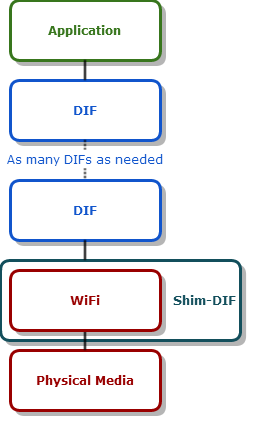
\includegraphics[width=0.4\textwidth]{figures/rinaoverwifi}
    \caption{RINA over WiFi} 
    \label{fig:rinaoverwifi}
\end{figure}
This is ultimately the question we are trying to answer. This question alone does not provide enough background and will need some further elaboration, which will be provided in this subsection. 
\npar
First we must note that RINA is the theory, actual working models are currently very scarce. We thus require a technical implementation of RINA. This will not be self constructed, we will be building further on a provided codebase. This project is \emph{Investigating RINA as Alternative to TCP/IP} (IRATI) \citep{vrijders2014prototyping}. This European project is a collaboration between: 
\begin{description}
	\item[i2CAT Foundation] \url{http://www.i2cat.net/en}
	\item[Nextworks] \url{http://www.nextworks.it}
	\item[iMinds] \url{http://www.iminds.be/en}
	\item[Interoute] \url{http://www.interoute.com/}
\end{description}
and is trying to bring a codebase for RINA upon which commercial implementations can be based. A working Recursive InterNetworking Architecture has already been developed for Linux operating systems. Since the Android platform is based on a trimmed and edited version of the Linux platform we will use the previously established code as a base. 
\npar

A current working Shim-DIF (more about specific working of RINA in \ref{ssec:RINAbasics}) has been constructed for 802.1Q (Ethernet) on Linux operating systems. A big portion of this research question is how to port the IRATI prototype on Android, more specifically to extend the prototype towards a working WiFi Shim-DIF. A key point for this Shim-DIF and the thesis as a whole is the need to be dependency free. When this Shim-DIF is dependency free it will guarantee the full and seamless working of RINA on mobile devices, specifically on the Android platform. Other physical connection mechanisms for Android such as: 3G, 4G, \ldots are not part of this thesis.
\npar
Another part of the research is dedicated towards the differences between the Linux and Android platform. Since IRATI is build in C in kernelspace and \cpp and Java in userspace.  These coding languages are well supported in Linux and in various other platforms. The issue here rises that the library that handles \cpp, \engels{glibc}, is not available in the Android operating system. On Android a variant of this library is available, called \engels{bionic}, this library however has more limited functionality, specifically some alterations on how \cpp is handled.
\npar
One final piece of research that will be completed is to figure out how to optimally map RINA API to the current WiFi standard. For this we will take a closer look at the current WiFi standard (802.11n) \citep{eldadperahia2008, sixtoortiz2009, thomaspaul2008}. We will examine the interaction this standard makes with several layers and where the Shim-DIF will some remodeling to seamlessly fit on the current WiFi standard.
\npar
This research question is now clearly stated and throughout this literature study we will try find the needed background information to help us formulate an answer in the thesis. The answer will not only be limited to pure text form, but shall also include working code for the prototype of the \emph{Shim-DIF over WiFi on Android}. 


\subsection{RINA basics and origin}
\label{ssec:RINAbasics}
Before we go any further we initiate with clearly stating what \engels{Recursive InterNetwork Architecture} (RINA) is, how it functions and what the origin of RINA is. As has been shown in subsection~\ref{ssec:Internet_shortcomings}, the current status of the Internet is facing a long list of issues. This is where RINA provides an adequate answer, it looks at previous network architectures and tries learn from those. In the end RINA proposes a basic, clear, and adequate answer for the networking needs.
\npar
RINA is a proposed architecture by John Day in his 2008 book: ``Patterns in Network Architecture: A return to fundamentals'' \citep{johnday2008}. 
Let us start by explaining the full name of RINA: \engels{Recursive InterNetwork Architecture}, first the last part: \engels{Architecture}, this states what the actual goal of this is. To implement an architecture that provides support for Network communication. One of the most important words in RINA is definitely: \engels{Recursive}. As can be seen in the IRATI symbol: a recursive tree. Recursive is defined as: ``pertaining to or using a rule or procedure that can be applied repeatedly.'' \citep{website:recursive_definition}, 
this instantly shows that the entire architecture is build on a base that can be repeated as many times as needed. It does not involve a static amount of layers, instead it can use as many or as few as needed to set up communication between two applications. The middle part: \engels{InterNetwork} shows that this architecture involves communication between and on networks and is not limited or restricted to single networks.
\npar
The main principle in RINA is that networking is simply and only: \engels{Inter-Process Communication} (IPC) \citep{johnday2008}. This is the premise on which entire RINA is founded on. An IPC is provided by IPC processes, a group of these coherent IPC processes forms a \engels{Distributed IPC Facility} (DIF) through enrollment. Every DIF is managed and has its own scope, it provides a way for processes to communicate between each other. DIFs have the same mechanism but are configured to different policies and thus have their own sets of rules. A DIF can ultimately be seen as a layer. For example the first DIF provides IPC directly to user applications. Below that you have a DIF that takes care of the communication between user A and the router user A is connected to. Every DIF has their own scope and once it becomes clear what the scope is for the DIF, the function of this DIF will be evident and be tailored to that scope. This repetition of DIFs goes on recursively until the entire chain of communication can be formed and finally the application from user A is interacting with the application from user B.
\npar
\begin{figure}[H]
    \centering
    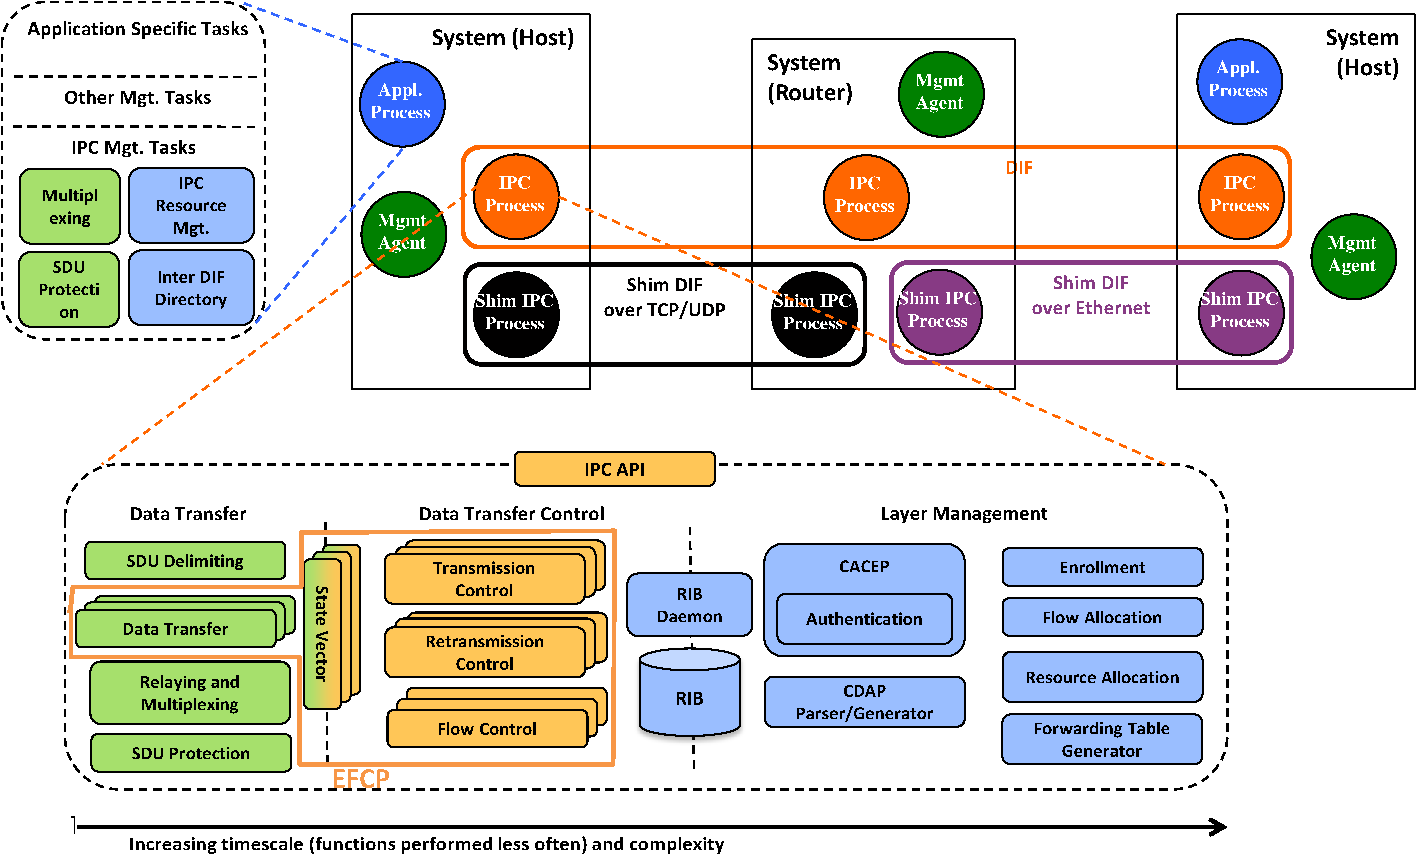
\includegraphics[width=\textwidth]{figures/referencemodel}
    \caption{Recursive InterNetworking Architecture example \citep{vrijders2014prototyping}} 
    \label{fig:RINAexample}
\end{figure}
\npar
An example how communication between two processes is established with RINA can be seen in the image~\ref{fig:RINAexample} above. Here we see application S on the host trying to communicate with application D on the other side of the communication chain. We see that for this specific example 3 levels of DIFs are used. These DIFs stack recursively from the bottom level (1st level) up till the DIF that actually takes care of the communication between the IPC and the application process. 
\npar
In this architecture we see that every application process, which also includes the IPC processes, has a name that is unique in that DIF. This is the way routing is ultimately done, but it no longer forces users to link applications to port numbers or specific IP addresses. While IP addresses can still be used in lower level DIFs for routing, the application does not to be aware of this. Naming stays within the DIF and is not visible outside that layer. In every DIF is a directory that contains these names of the IPC process names  and associates these to the application names (layer above the DIF). This is where we instantly see the possibility for multihoming. One application name can have different IPC processes in the layer below, but due to the design this application process does not need to be aware of this. The architecture will choose the most optimal routing and provide communication between the application processes in the layer above that requested it. Finally we must name the way a DIF sees it's surroundings. A DIF on the layer above is named the application. The process below the DIF is called the Point of Attachment. 


\subsection{IRATI implementation}

In this part we will address the technical implementation of the RINA model. The implementation that we will be using is developed in the IRATI project. 
\\
In this subsection we will further explain the current development status of IRATI, the future goals and give a brief explanation of the technical aspects of this project.
\npar
The IRATI project is building a working, open source, technical implementation of the Recursive InterNetwork Architecture in Linux with parts in both kernel and userspace\citep{website:IRATI-obj}. The technical roadmap towards this goal has been divided in 3 parts. 

\begin{enumerate}
	\item Restricted prototype (November 2013)
	\item Open source prototype (June 2014)
	\item Open source prototype, further development (December 2014)
\end{enumerate}

These different phases show the current plan of action for the project. They represent the coarse lines along which the project will guide itself. More specifically the project aims to have a technical implementation that features both parts in kernel space and in user space. These should be loosely coupled and functionalities that take part in both user and kernel space should be avoided. The reason that this currently has to be done is that for the entire architecture to work optimally we would need to have a brand new kernel based on this architecture. This is not within the confinement of the project and thus IRATI opts for a loosely coupled, although less optimal, system. Within this project is also a big part that represents the application programmable interface (API), this is fits itself within the user space. It acts as an adaptor in the project and presents the RINA stack towards the applications as a common interface. This is of utmost importance because thanks to this the applications quickly become versatile and cross platform. When the same API functions are offered on different platforms it becomes irrelevant for the application which operating system it is running on. As long as API functions presented to the the applications stay the same. This API currently offers bindings for C and \cpp for the applications. However bindings for other programming languages can be quickly implemented when using tools such as SWIG. SWIG stands for Simplified Wrapper and Interface Generator and can, when prompted present the C/\cpp bindings as other programming language bindings. A working example of this is the currently operational Java bindings for RINA. 

\npar

The first phase of the project focuses on having a working prototype of RINA. This prototype should be as low as possible within the current Internet stack. Due to not being able to fully redevelop a brand new kernel, outside the project's scope, the option has been made that the lowest feasible is the Ethernet stack. More specifically virtual LAN (vlan) Ethernet, 802.1Q. This requires one special DIF, a Shim-DIF over Ethernet that presents Ethernet in such a way that DIFs on top of this Shim-DIF can use it as part of RINA. This entire architecture is presented in the following figure~\ref{fig:rinaoverethernet}. This provides a technical proof-of-concept for RINA. It will also add functionality to current Internet, such as multihoming and improved mobility \citep{vrijders2014prototyping}. During this phase of the project the code is not publicly available.

\npar
\begin{figure}[H]
    \centering
    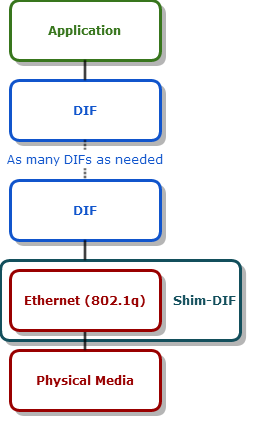
\includegraphics[width=0.4\textwidth]{figures/rinaoverethernet}
    \caption{Recursive InterNetworking Architecture example over Ethernet} 
    \label{fig:rinaoverethernet}
\end{figure}

\npar

After the first phase of the project has been completed and several iterations over the current code have been completed, it can move towards the open source phase. This should be around June 2014. In this phase functionality should be supplemented to the existing codebase. Not only should the previously working parts of the project be improved upon and publicly released, but new functionalities should be added. These items can be different levels of support on top of different layers of the current Internet. Expansions could be made towards other protocols than UDP or IP. Other platforms could be explored such as Android which is a minimal deviation from the current Linux Operating Systems that are being focused on. 

\npar
The final phase is to further iterate upon the currently existing codebase. This means fixing bugs and further improving functionality. These steps lead towards a well-developed technical project that clearly shows a proper implementation of RINA. During this phase further spread towards other operating systems and protocols is the main target. This will lead to a strong interoperability between different architectures and protocols using RINA. From the second phase on the project will be open sourced and aim to set up a strong developing community around the technical implementation of RINA. 

\npar

Finally we will briefly touch on how the thesis utilises the IRATI project. The thesis is focused on the WiFi implementation on Android operating systems (figure~\ref{fig:rinaoverwifi}). More specifically the thesis will aim to port the IRATI stack on the Android platform over WiFi. For this code will be used that was produced during the first phase. The code will be made publicly available when the second phase is reached, which should be at the end of this Master Thesis. 


